\begin{mydef}
	\iftoggle{eleve}{%
		Deux droites sont\vspace*{0.2cm}
		\hrulefill
		
		\vspace*{0.2cm}
		\hrulefill
		
		\vspace*{0.2cm}
		\hrulefill
		
		
	}{%
	Deux droites sont \kw{sécantes} si elles n'ont qu'un seul point commun : leur \kw{point d'intersection}.
}
\end{mydef}



\begin{myex}
	\begin{multicols}{2}
		
		\iftoggle{eleve}{%
		Les droites $(d)$ et $(d')$ sont \\
	}{%
		Les droites $(d)$ et $(d')$ sont sécantes en $O$, leur point d'intersection.1
}
		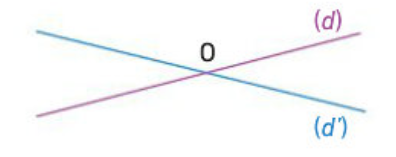
\includegraphics[scale=0.13]{img/sec}
	\end{multicols}
	
\end{myex}

\begin{mydef}
	\iftoggle{eleve}{%
	\vspace*{0.2cm}
	Deux droites $(d_1)$ et $(d_2)$ sont\hrulefill
	
	\vspace*{0.2cm}
	\hrulefill
	
	\vspace*{0.2cm}
	\hrulefill
	
	
}{%	
	Deux droites $(d_1)$ et $(d_2)$ sont \kw{perpendiculaires} si elles se coupent en formant \kw{quatre angles droits}. On note $(d_1) \perp (d_2)$.
}
\end{mydef}

\begin{myex}
	\begin{multicols}{2}
		\iftoggle{eleve}{%
			Les droites $(d_1)$ et $(d_2)$ sont \\
			
		}{%
			Les droites $(d_1)$ et $(d_2)$ sont perpendiculaires en $A$. %$A$ est le pied de la perpendiculaire à $(d')$.
}
		
		
		\begin{center}
			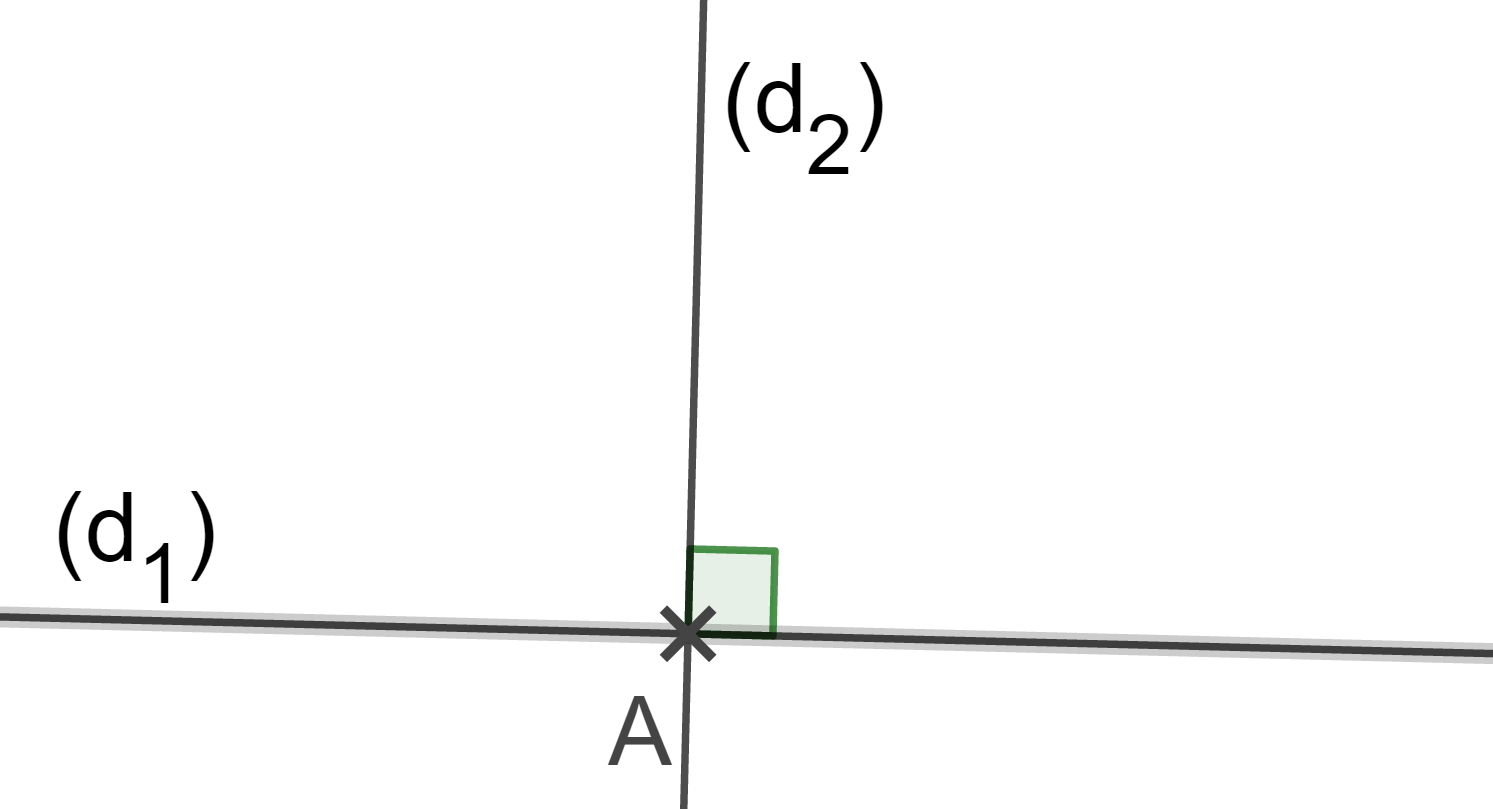
\includegraphics[scale=0.13]{img/perp}
		\end{center}
		
	\end{multicols}
	
\end{myex}

\begin{mydef}
	\iftoggle{eleve}{%
	\vspace*{0.2cm}
	Deux droites $(d_3)$ et $(d_4)$\hrulefill
	
	\vspace*{0.2cm}
	\hrulefill
	
	\vspace*{0.2cm}
	\hrulefill
	
	
}{%	
	Deux droites $(d_3)$ et $(d_4)$ qui ne sont pas sécantes sont \kw{parallèles}. On note $(d_3) // (d_4)$.
}
\end{mydef}

\begin{myex}
	\begin{multicols}{2}
		\iftoggle{eleve}{%
			Les droites $(d_3)$ et $(d_4)$ sont	
		}{%
		Les droites $(d_3)$ et $(d_4)$ sont parallèles. Même en les prolongeant à l'infini elles ne se rencontreront jamais.
	}
		
		
		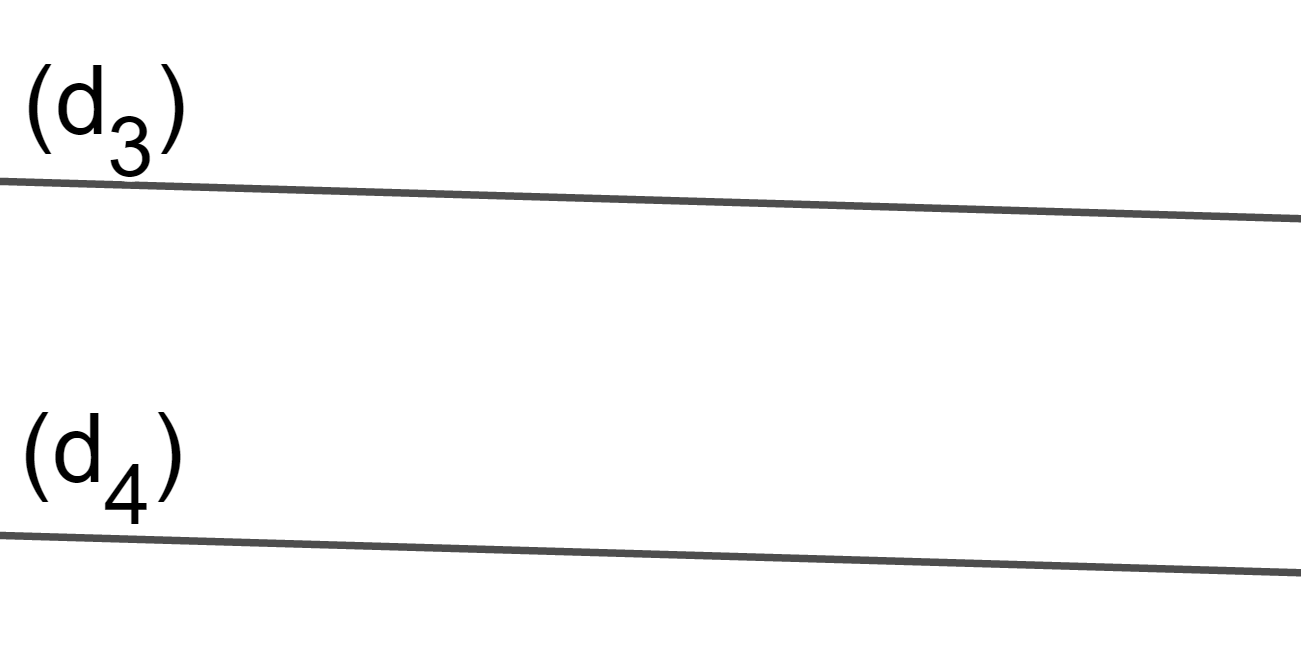
\includegraphics[scale=0.13]{img/para1}
	\end{multicols}
	
\end{myex}



